%%%%%%%%%%%%%%%%%%%%%%%%%%%%%%%%%%%%%%%%%%%%%%%%%%%
%
%  New template code for TAMU Theses and Dissertations starting Fall 2016.
%
%
%  Author: Sean Zachary Roberson
%  Version 3.17.09
%  Last Updated: 9/21/2017
%
%%%%%%%%%%%%%%%%%%%%%%%%%%%%%%%%%%%%%%%%%%%%%%%%%%%
%%%%%%%%%%%%%%%%%%%%%%%%%%%%%%%%%%%%%%%%%%%%%%%%%%%%%%%%%%%%%%%%%%%%%%
%%                           SECTION III
%%%%%%%%%%%%%%%%%%%%%%%%%%%%%%%%%%%%%%%%%%%%%%%%%%%%%%%%%%%%%%%%%%%%%

\chapter{UNSTRUCTURED MESHING AND LOAD BALANCING IN PDT}\label{cha:lb}

Initially, PDT only swept on structured, logically Cartesian meshes. As the need to solve problems with more complex geometries arose, PDT added a support for arbitrary polyhedral unstructured meshes. However, this introduced imbalanced partitions (or different amounts of cells per processor), causing longer and unmanageable runtimes.

To combat imbalanced partitions, two load balancing algorithms were implemented, referred to in this thesis as the original load-balancing algorithm \cite{mastersthesis,mc2017} and the load-balancing-by-dimension algorithm.

Before detailing the two load balancing algorithms PDT employs, a quick review of partitioning unstructured meshes in PDT is necessary:
\begin{itemize}
\item ``Cut lines'' in 2D (``cut planes'' in 3D) are used to slice through the mesh in the $x$, $y$, and $z$ dimensions.
\item The cut planes form brick partitions, called subsets, that have unstructured meshes inside of them.
\item Discontinuities along subset boundaries are fixed by ``stitching'' hanging nodes, creating degenerate polygons along subset boundaries.
\item The subsets are distributed amongst the processor domain.
\end{itemize}
Using cut lines/cut planes to partition unstructured meshes may preserve the provably optimal sweep partitioning \cite{mpadams2013,mpadams2015} of logically Cartesian grids if each partition has an equivalent number of cells.
Subsets, rather than the cells, have $(i,j,k)$ indices and will become the base unit when aggregating spatial parameters. That is, $A_x$ and $A_y$ will now represent the number of subsets in $x$ and $y$ aggregated into a task.
Generally, one subset is assigned per processor, as this minimizes the communication costs across processor boundaries, although this is not required. \jcr{FROM TAREK: processor connection shown here}\jcr{where?}
Figure~\ref{partitioning_example} shows an example of an unstructured mesh partitioned into 100 subsets in PDT.
\begin{figure}[H]
\centering
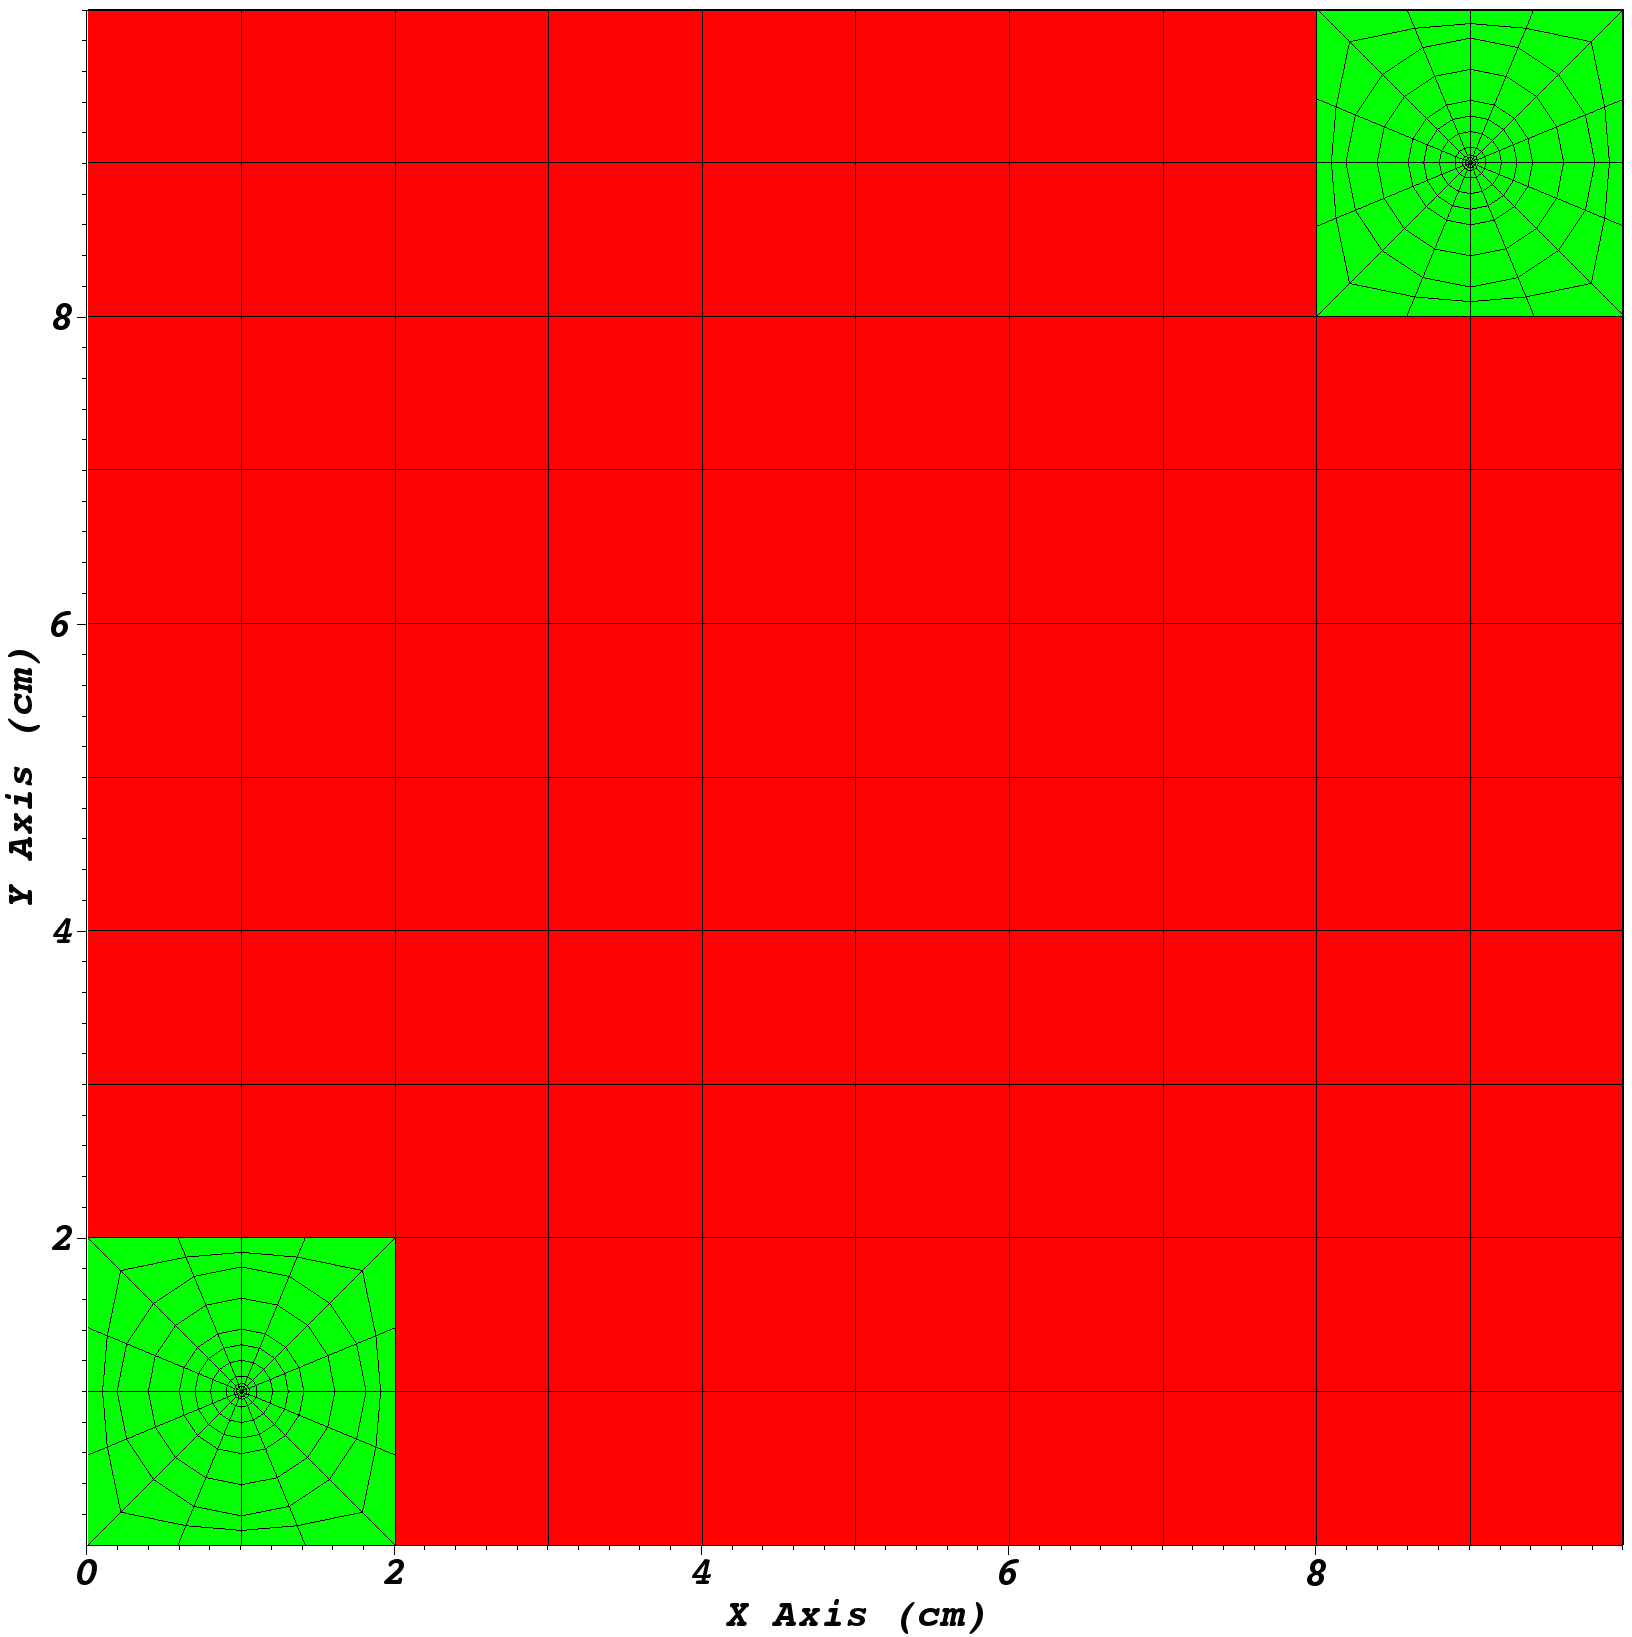
\includegraphics[scale=0.2]{../figures/spiderweb_10x10_sparse.png}
\caption{An unstructured mesh partitioned into 100 subsets with cut lines at 1 cm intervals in both dimensions}
\label{partitioning_example}
\end{figure}

Upon creation, the subsets may have geometric discontinuities as a result of slicing through the mesh.
Figure~\ref{hanging_node} shows an example of a hanging node across a subset boundary.
This node is stitched across the boundary to preserve geometric continuity, forming a degenerate polygon \cite{degenerate} (in Fig.~\ref{hanging_node}, a degenerate square).
PDT uses Piece-Wise Linear Discontinuous (PWLD) finite-element basis functions \cite{pwld_ragusa,pwld_teresa} that allow for solutions on arbitrary and degenerate polyhedra.
\begin{figure}[H]
  \centering
  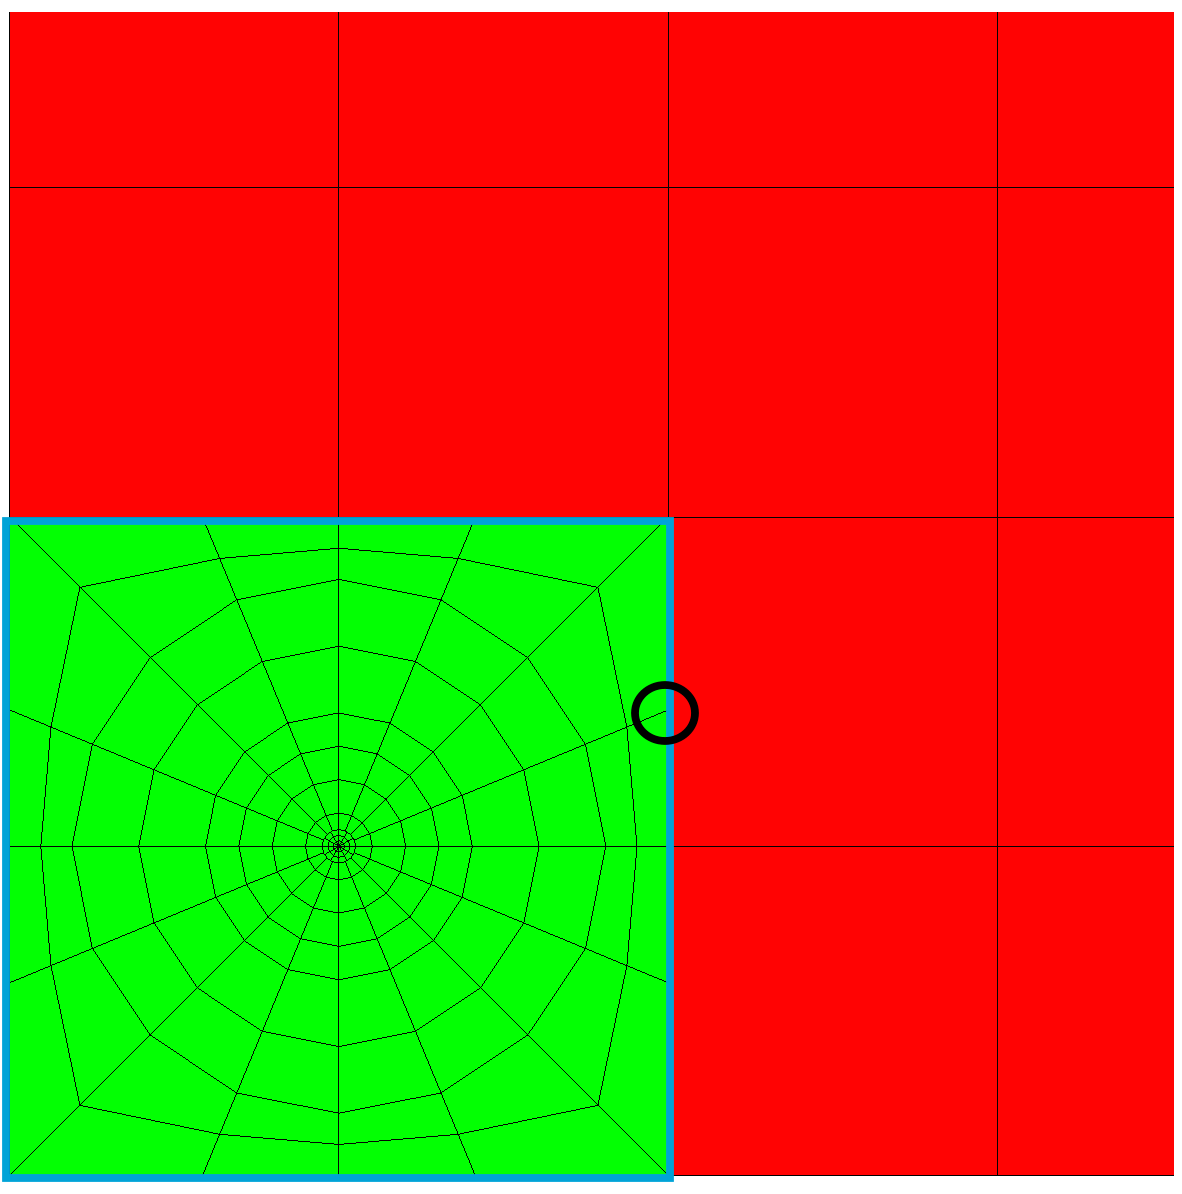
\includegraphics[scale=0.2]{../../figures/hanging_node_spiderweb_example.png}
   \caption{A hanging node (circled in black) on a subset boundary (highlighted in blue).}
   \label{hanging_node}
\end{figure}

Both approaches to load balancing move cut lines in order to redistribute cells more evenly throughout subsets. We define a metric describing how imbalanced our problem is:
\begin{equation}
f =\frac{\underset{ijk}{\text{max}}(N_{ijk})}{\frac{N_{tot}}{I\cdot J\cdot K}},
\label{metric_def}
\end{equation}
where $f$ is the load balance metric, $N_{ijk}$ is the number of cells in subset $(i,j,k)$, $N_{tot}$ is the global number of cells in the problem, and $I$, $J$, and $K$ are the total number of subsets in the $x$, $y$, and $z$ directions, respectively. The metric is a measure of the maximum number of cells per subset divided by the average number of cells per subset. For a perfectly balanced problem, $f = 1$.

Figure~\ref{redistribute} illustrates an example of redistributing the cut planes in $x$ to balance the cells per column.
\begin{figure}[H]
\centering
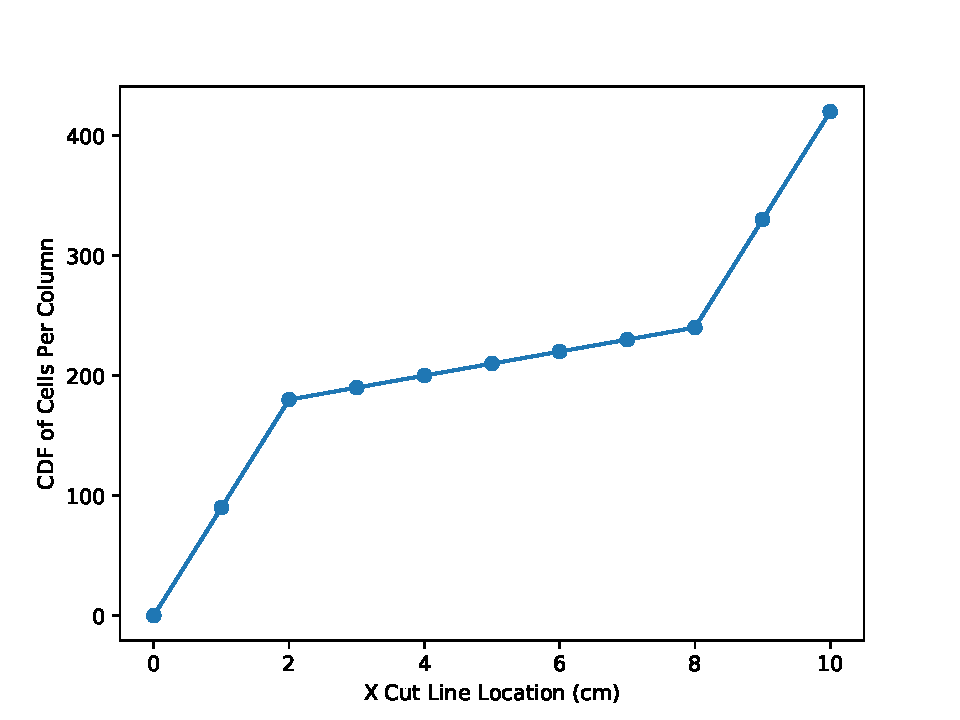
\includegraphics[scale=0.4]{../figures/spiderweb_redistribute_before_sparse.pdf}
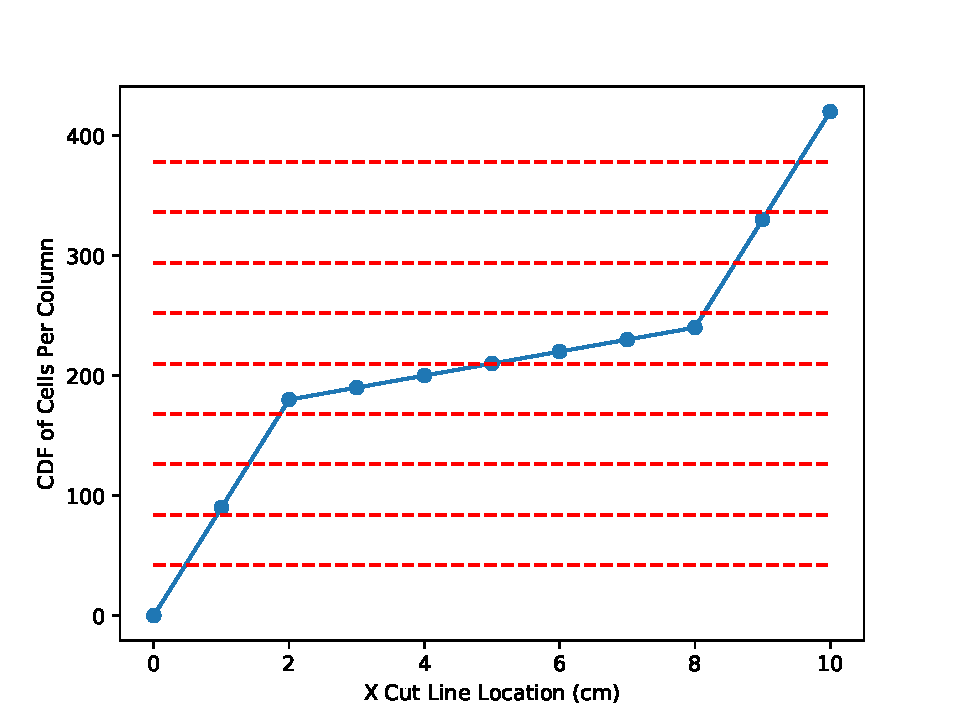
\includegraphics[scale=0.4]{../figures/spiderweb_redistribute_after_sparse.pdf}
\caption{The use of the CDF of cells per column to redistribute the cut lines in X.}
\label{redistribute}
\end{figure}
The image on the left side of Fig.~\ref{redistribute} shows the CDF of the cells per column in Fig.~\ref{partitioning_example}. The red lines on the right side of Fig.~\ref{redistribute} show the ideal equal number of cells per column. The x-value of the intersection of these red lines and the CDF are where the cut lines are redistributed to.

In order to decide the necessity of redistributing a dimension's cut lines/planes, we use dimensional sub-metrics of the following form:
\begin{equation}
f_{Z} = \frac{\underset{k}{\text{max}}[\sum_{i,j} N_{ijk}]}{\frac{N_{tot}}{K}},
\label{f_z}
\end{equation}
where $K$ is the total number of z-planes.
Equation \ref{f_z} is a metric defining how imbalanced the problem's planes are. It calculates the maximum cells per plane divided by the average cells per plane. If $f_K$ is greater than a predefined tolerance, the z cut planes are redistributed using the process in Fig.~\ref{redistribute}.

\section{Original Load-Balancing Algorithm}
\label{sec:og_lb}

The initial approach to load balancing was implemented on 2D extruded meshes, meaning the mesh is balanced in the 2D plane and then extruded, yielding a balanced 3D mesh. The metrics for this algorithm are defined as follows:
\begin{align}
f &= \frac{\underset{ij}{\text{max}}(N_{ij})}{\frac{N_{tot}}{I\cdot J}}  \label{og_metric}\\
f_X &= \frac{\underset{i}{\text{max}}[\sum_{j} N_{ij}] } {\frac{N_{tot}}{I}} \label{og_i_metric} \\
f_Y &= \frac{\underset{j}{\text{max}}[\sum_{i} N_{ij}] } {\frac{N_{tot}}{J}} \label{og_j_metric}
\end{align}
Equation \ref{og_metric} mirrors Eq. \ref{metric_def} for 2 dimensions, and Eqs. \ref{og_i_metric} and \ref{og_j_metric} define the column and row-wise metrics respectively.

 Algorithm \ref{initial_algorithm} summarizes the original approach to load balancing meshes in PDT.
\begin{algorithm}[H]
\caption{The original load-balancing algorithm.}
\label{initial_algorithm}
\begin{algorithmic}

\WHILE{$f > 1 + \text{tol}_{\text{subset}}$}
  \IF {$f_X > 1 + \text{tol}_{\text{col}}$}
    \STATE Redistribute the X cut lines.
  \ENDIF
  \IF {$f_Y > 1 + \text{tol}_{\text{row}}$}
  	\STATE Redistribute the Y cut lines.
  \ENDIF
\ENDWHILE
\end{algorithmic}
\end{algorithm}
While the problem is not balanced:
\begin{itemize}
  \item Check if the columns are balanced, and if not redistribute the X cut lines.
  \item Check if the rows are balanced, and if not redistribute the Y cut lines.
  \item Repeat until the mesh is balanced or until a maximum number of iterations is reached.
\end{itemize}

The original load-balancing algorithm placed cut lines in all dimensions all the way through the mesh.
This created an orthogonal partitioning where each subset had an equivalent number of neighbors, which was done to preserve the provably optimal sweep partitioning described by Adams et. al \cite{mpadams2013,mpadams2015}.
However, there are theoretical limits to load balancing in this fashion. Figure~\ref{2dgeneral} shows a simple 2D subset layout with $M$ unaligned patches with $N$ cells each.

\begin{figure}[H]
\centering
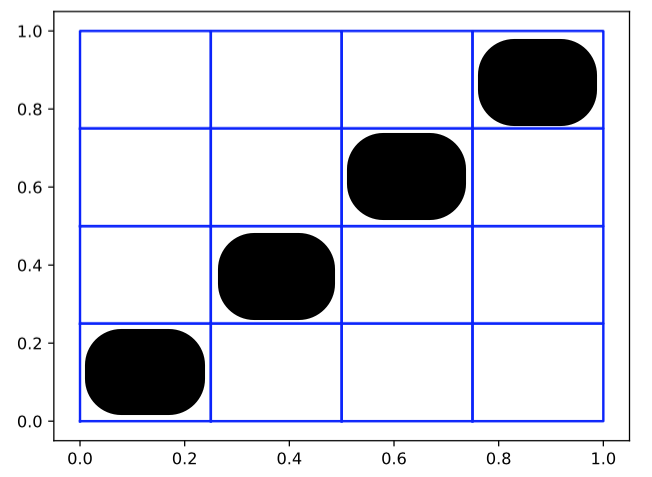
\includegraphics[scale=0.4]{../figures/theoretical_plot.png}
 \caption{A 2D subset layout with $M$ unaligned patches of high mesh density $N$.}
\label{2dgeneral}
\end{figure}
The subset layout is $M^2$, but only $M$ subset have significant work, leading to a theoretical limit for the load imbalance factor:
\begin{equation}
f= \frac{N}{(MN+C)/M^2} \xrightarrow{N\to \infty} \frac{N}{N/M} = M.
\end{equation}
Due to this theoretical limit, the load-balancing-by-dimension algorithm was developed.

\section{Load-Balancing-by-Dimension Algorithm}
\label{sec:lbd}

The load-balancing-by-dimension by dimension (LBD) algorithm, similar to the original load-balancing algorithm, relies on the movement of cut lines/planes to redistribute mesh cells in a more balanced manner.
However, cut lines are no longer required to go all the way through the mesh, and the load-balancing-by-dimension algorithm is fully extensible to 3 dimensions.
The load-balancing-by-dimension algorithm is summarized by:
\begin{enumerate}
  \item Slice the mesh in $z$ and redistribute cut planes until each plane has approximately an equivalent number of cells.
  \item For each $z$ layer, slice the layer in columns and redistribute the $x$ cut lines until each column has an approximately equivalent number of cells.
  \item For each column within each $z$ layer, slice the column in rows and redistribute the $y$ cut lines until each row has an approximately equivalent number of cells.
\end{enumerate}

We once again use dimensional sub-metrics to determine whether or not a dimension's cut lines/planes need to be redistributed. The $z$ dimension's sub-metric is defined by Eq. \ref{f_z}. For the LBD algorithm, there are $K$ column-wise metrics, one for each $z$ layer:
\begin{equation}
f_{X,k} = \frac{ \underset{i}{\text{max}}[ \sum_{j} N_{ijk}]  }  {\frac{N_{tot,k}}{I}},
\label{lbd_x_metric}
\end{equation}
where $N_{tot,k}$ is the number of cells in layer $k$.
Equation \ref{lbd_x_metric} defines the column-wise metric for layer $k$, or the maximum number of cells per column in layer $k$ divided by the average number of cells per column in layer $k$.

For the LBD algorithm, there are $K\cdot I$ row-wise metrics, one for each column in each $z$ layer:
\begin{equation}
f_{Y,k,i} = \frac{\underset{j}{\text{max}} N_{ijk} } {\frac{N_{tot,k,i}}{J}},
\label{lbd_y_metric}
\end{equation}
where $N_{tot,k,i}$ is the number of cells in column $i$ in layer $k$.
Equation \ref{lbd_y_metric} defines the row-wise metric for layer $k$ in column $i$, or the maximum number of cells per row in column $i$ in layer $k$ divided by the average number of cells per row in column $i$ in layer $k$.

Algorithm \ref{lbd} details the load-balancing-by-dimension algorithm.
\begin{algorithm}[H]
\caption{The load-balancing-by-dimension algorithm.}
\label{lbd}
\begin{algorithmic}

  \WHILE {$f_{Z} > 1 + \text{tol}_{\text{K}}$}
    \STATE Redistribute the Z cut planes.
  \ENDWHILE

  \FOR {$k$ in $K$}
    \WHILE {$f_{X,k} > 1 + \text{tol}_{\text{I}}$}
      \STATE Redistribute the X cut lines within layer $k$.
    \ENDWHILE
  \ENDFOR

  \FOR{$k$ in $K$}
    \FOR{$i$ in $I$}
      \WHILE {$f_{Y,k,i} > 1 +  \text{tol}_{\text{J}}$ }
        \STATE Redistribute the Y cut lines in column $i$ in layer $k$.
      \ENDWHILE
    \ENDFOR
  \ENDFOR

  \STATE Calculate $f$.
\end{algorithmic}
\end{algorithm}

\jcr{what’s the connection with the processor layout. at some point, it is good to loop back on that notion that was heavily present before and now has disappeared}

Figure~\ref{alg_illustration} illustrates the behavior of both algorithms after 5 iterations. In Fig.~\ref{3x3_lb}, we see the partitions cutting across the entire domain, with the $x$ and $y$ cut lines moving into the denser geometric features in the corners to more evenly distribute cells. In Fig.~\ref{3x3_lbd}, we see the $x$ partitions cutting across the entire domain, but the $y$ partitions being redistributed by column. The $y$ partitions are moved into the respective geometric features in the appropriate columns in order to better balance the problem.

\begin{figure}[H]
\centering
\begin{subfigure}[t]{\textwidth}
\centering
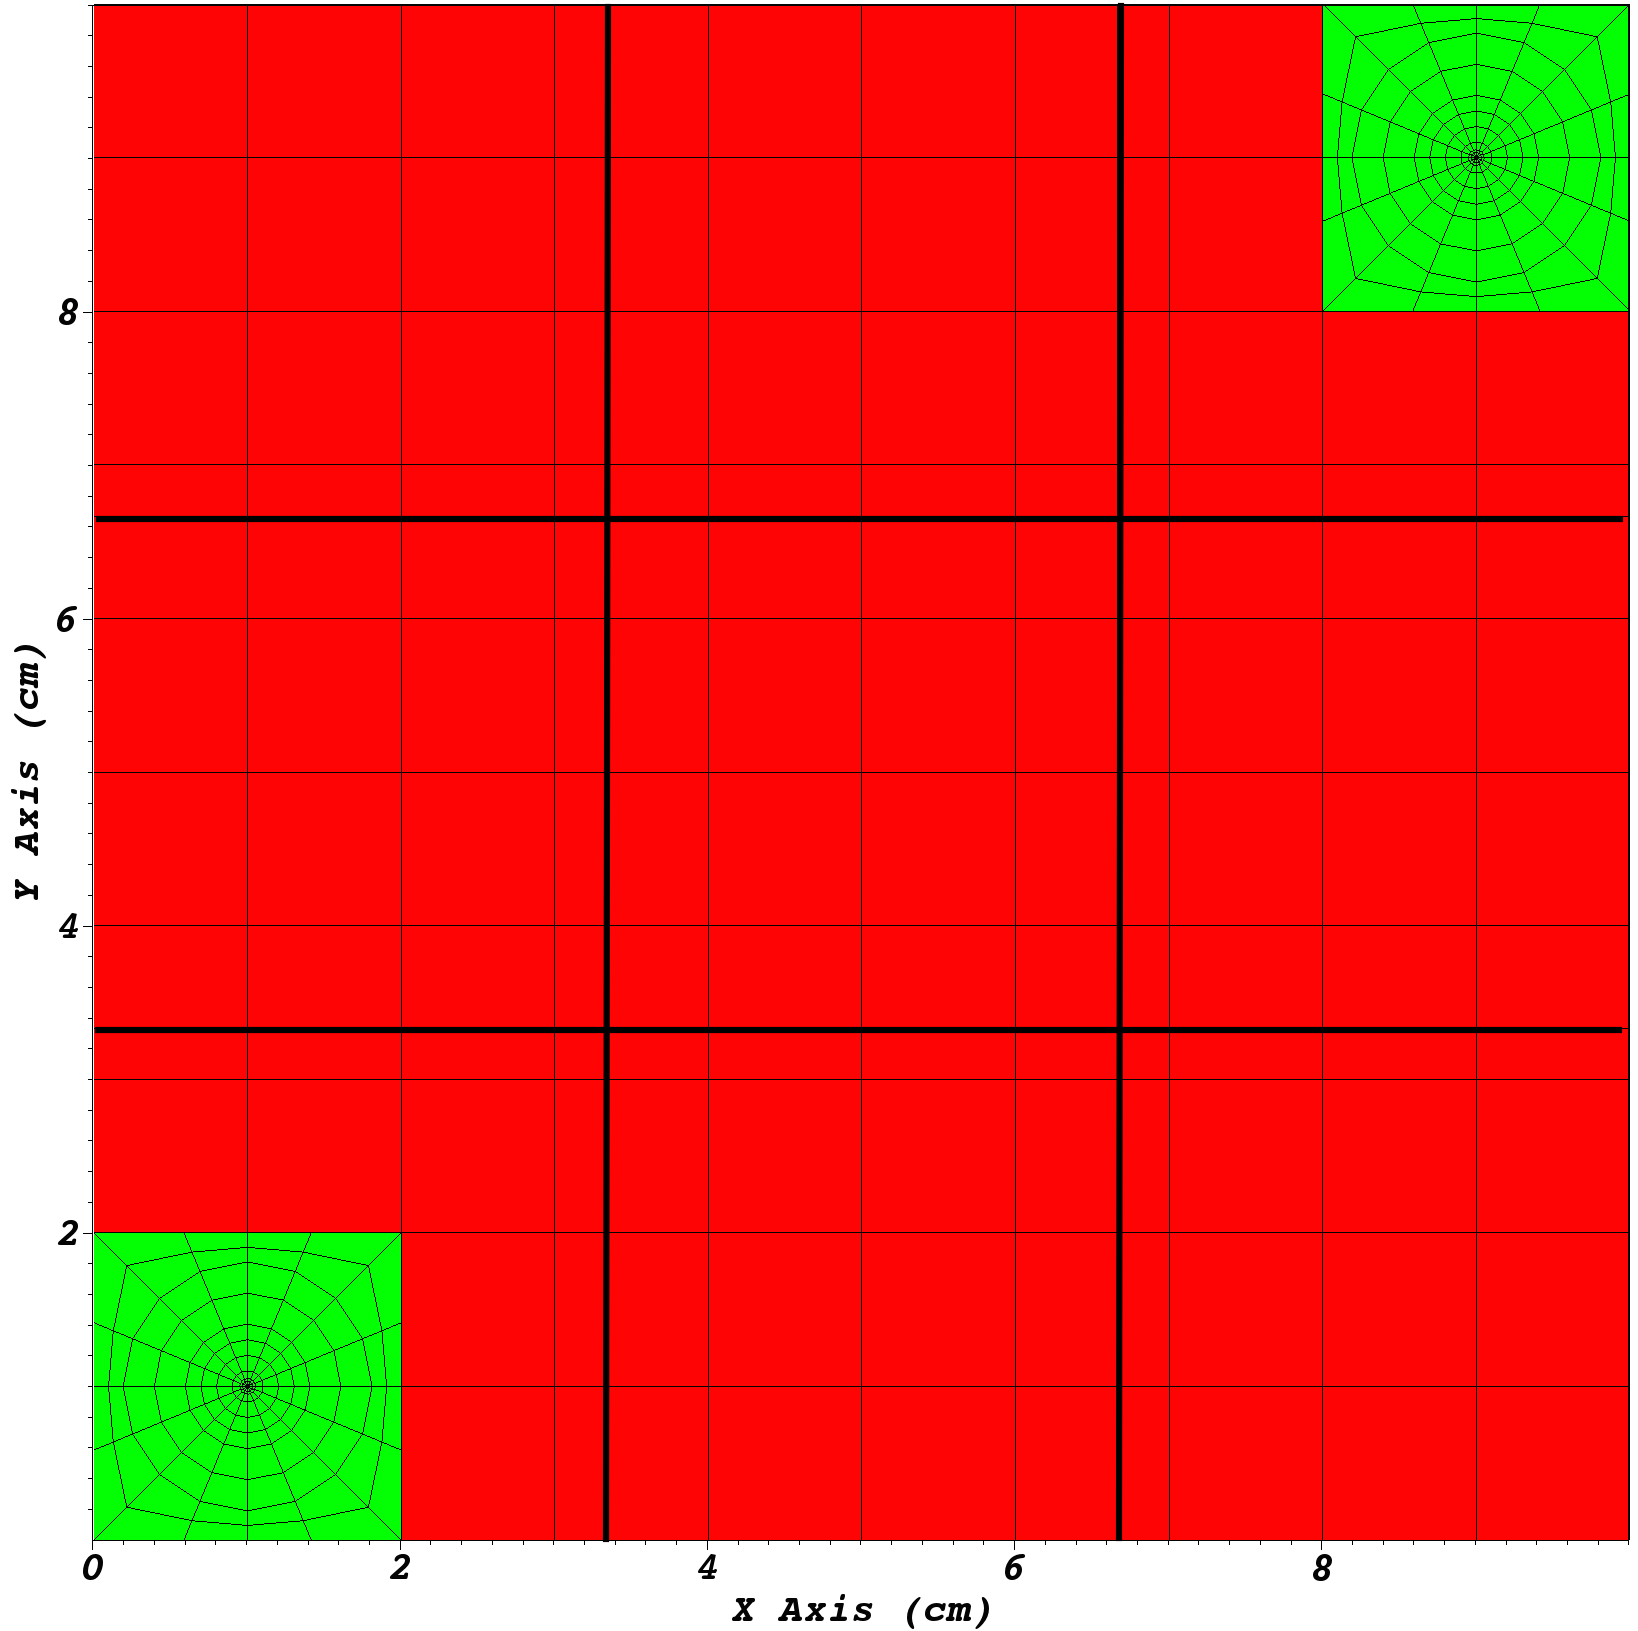
\includegraphics[scale=0.15]{../figures/ubp_3x3_regular.png}
\caption{No load balancing, $f = 3.41$.}
\label{3x3_regular}
\end{subfigure}
\begin{subfigure}[b]{0.49\textwidth}
\centering
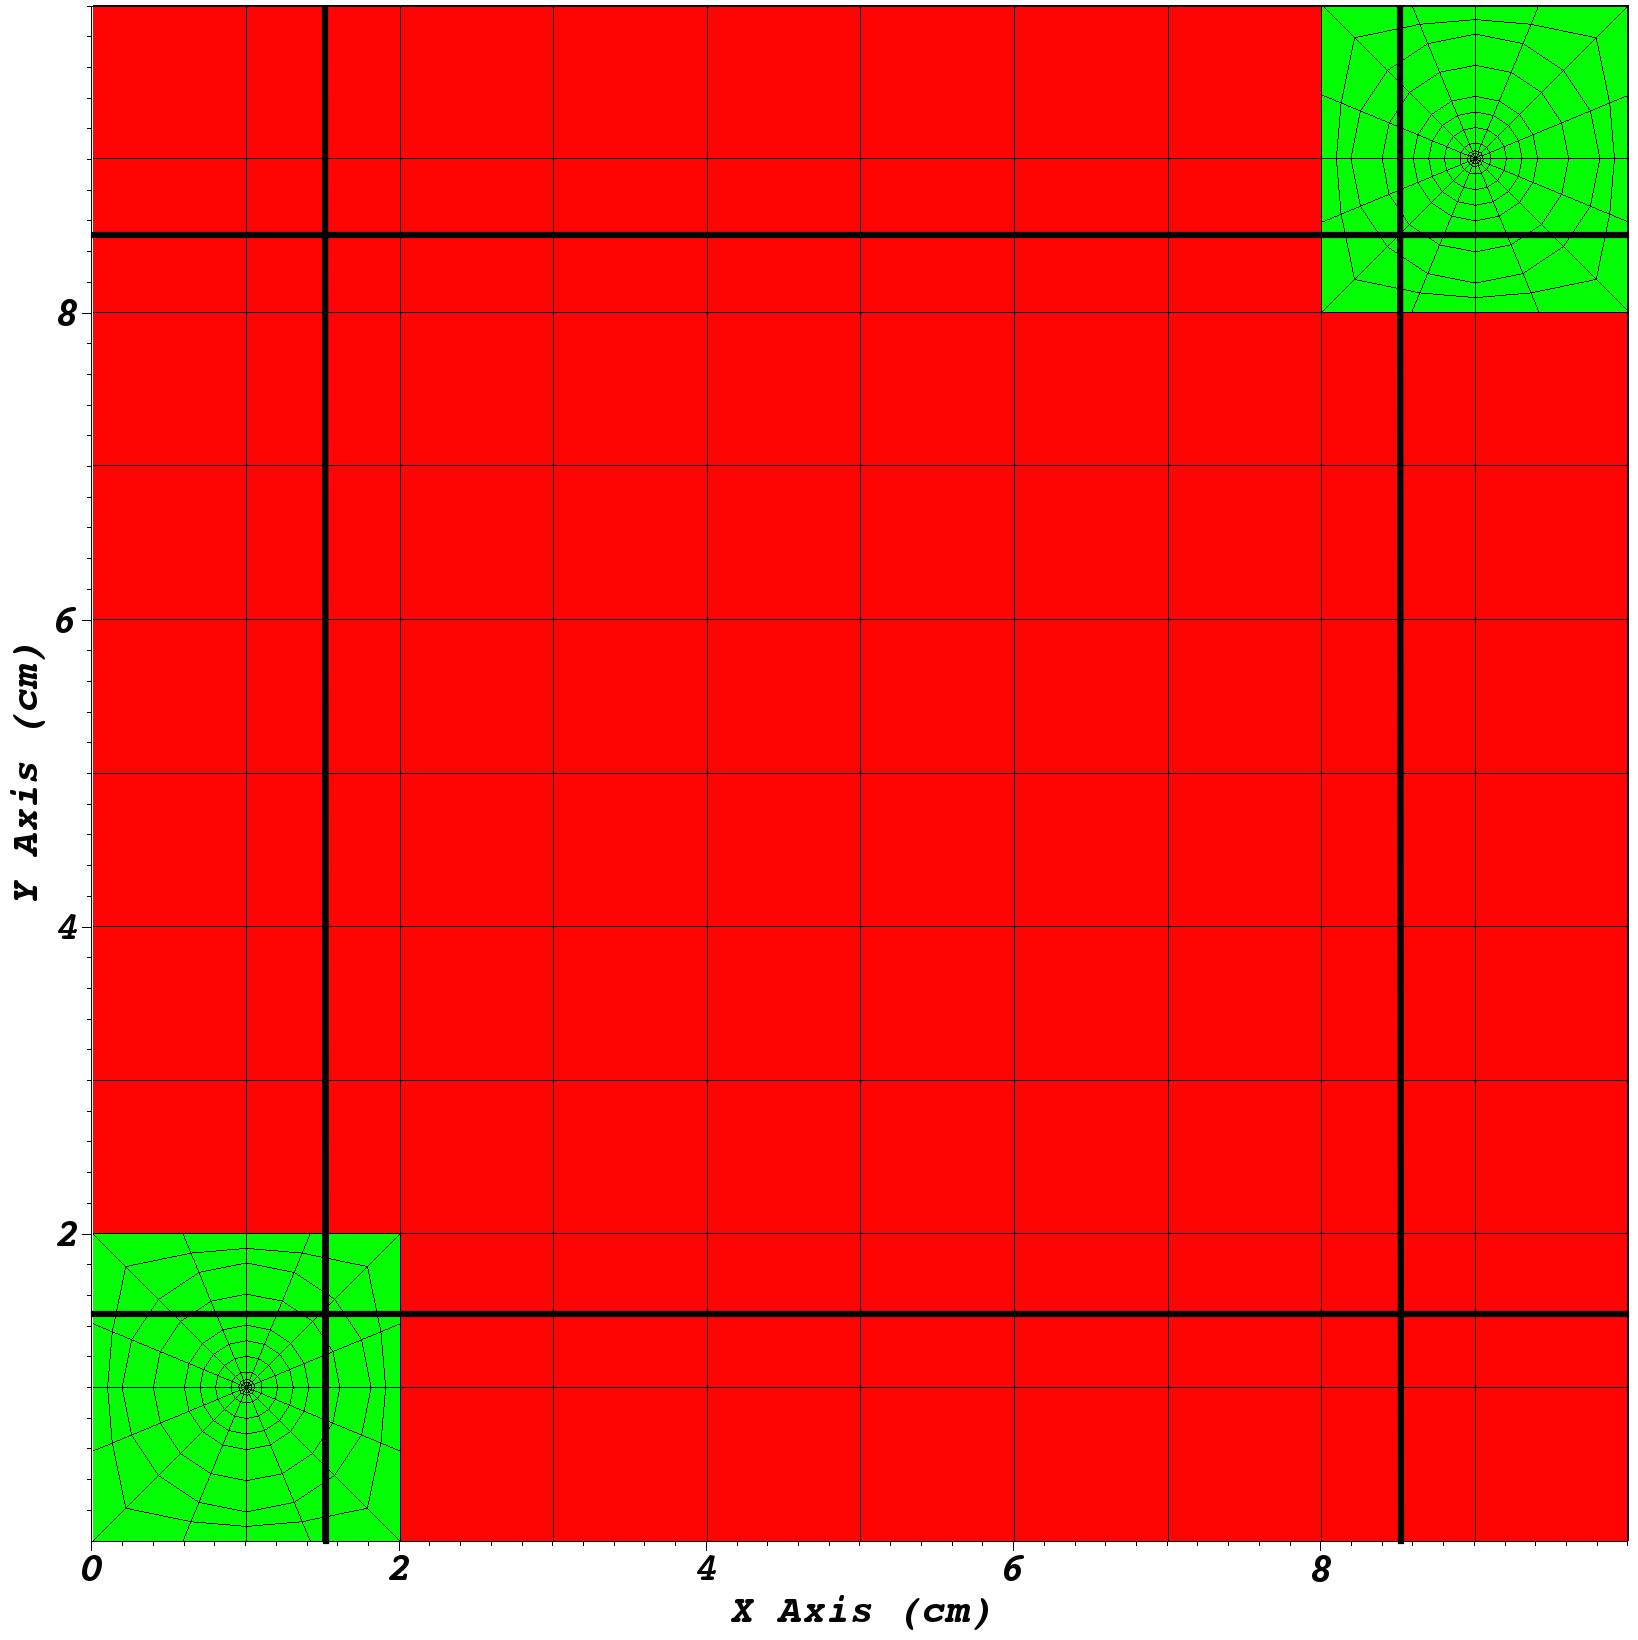
\includegraphics[scale=0.13]{../figures/ubp_3x3_lb.png}
\caption{5 load balancing iterations, $f = 2.58$.}
\label{3x3_lb}
\end{subfigure}
\begin{subfigure}[b]{0.49\textwidth}
\centering
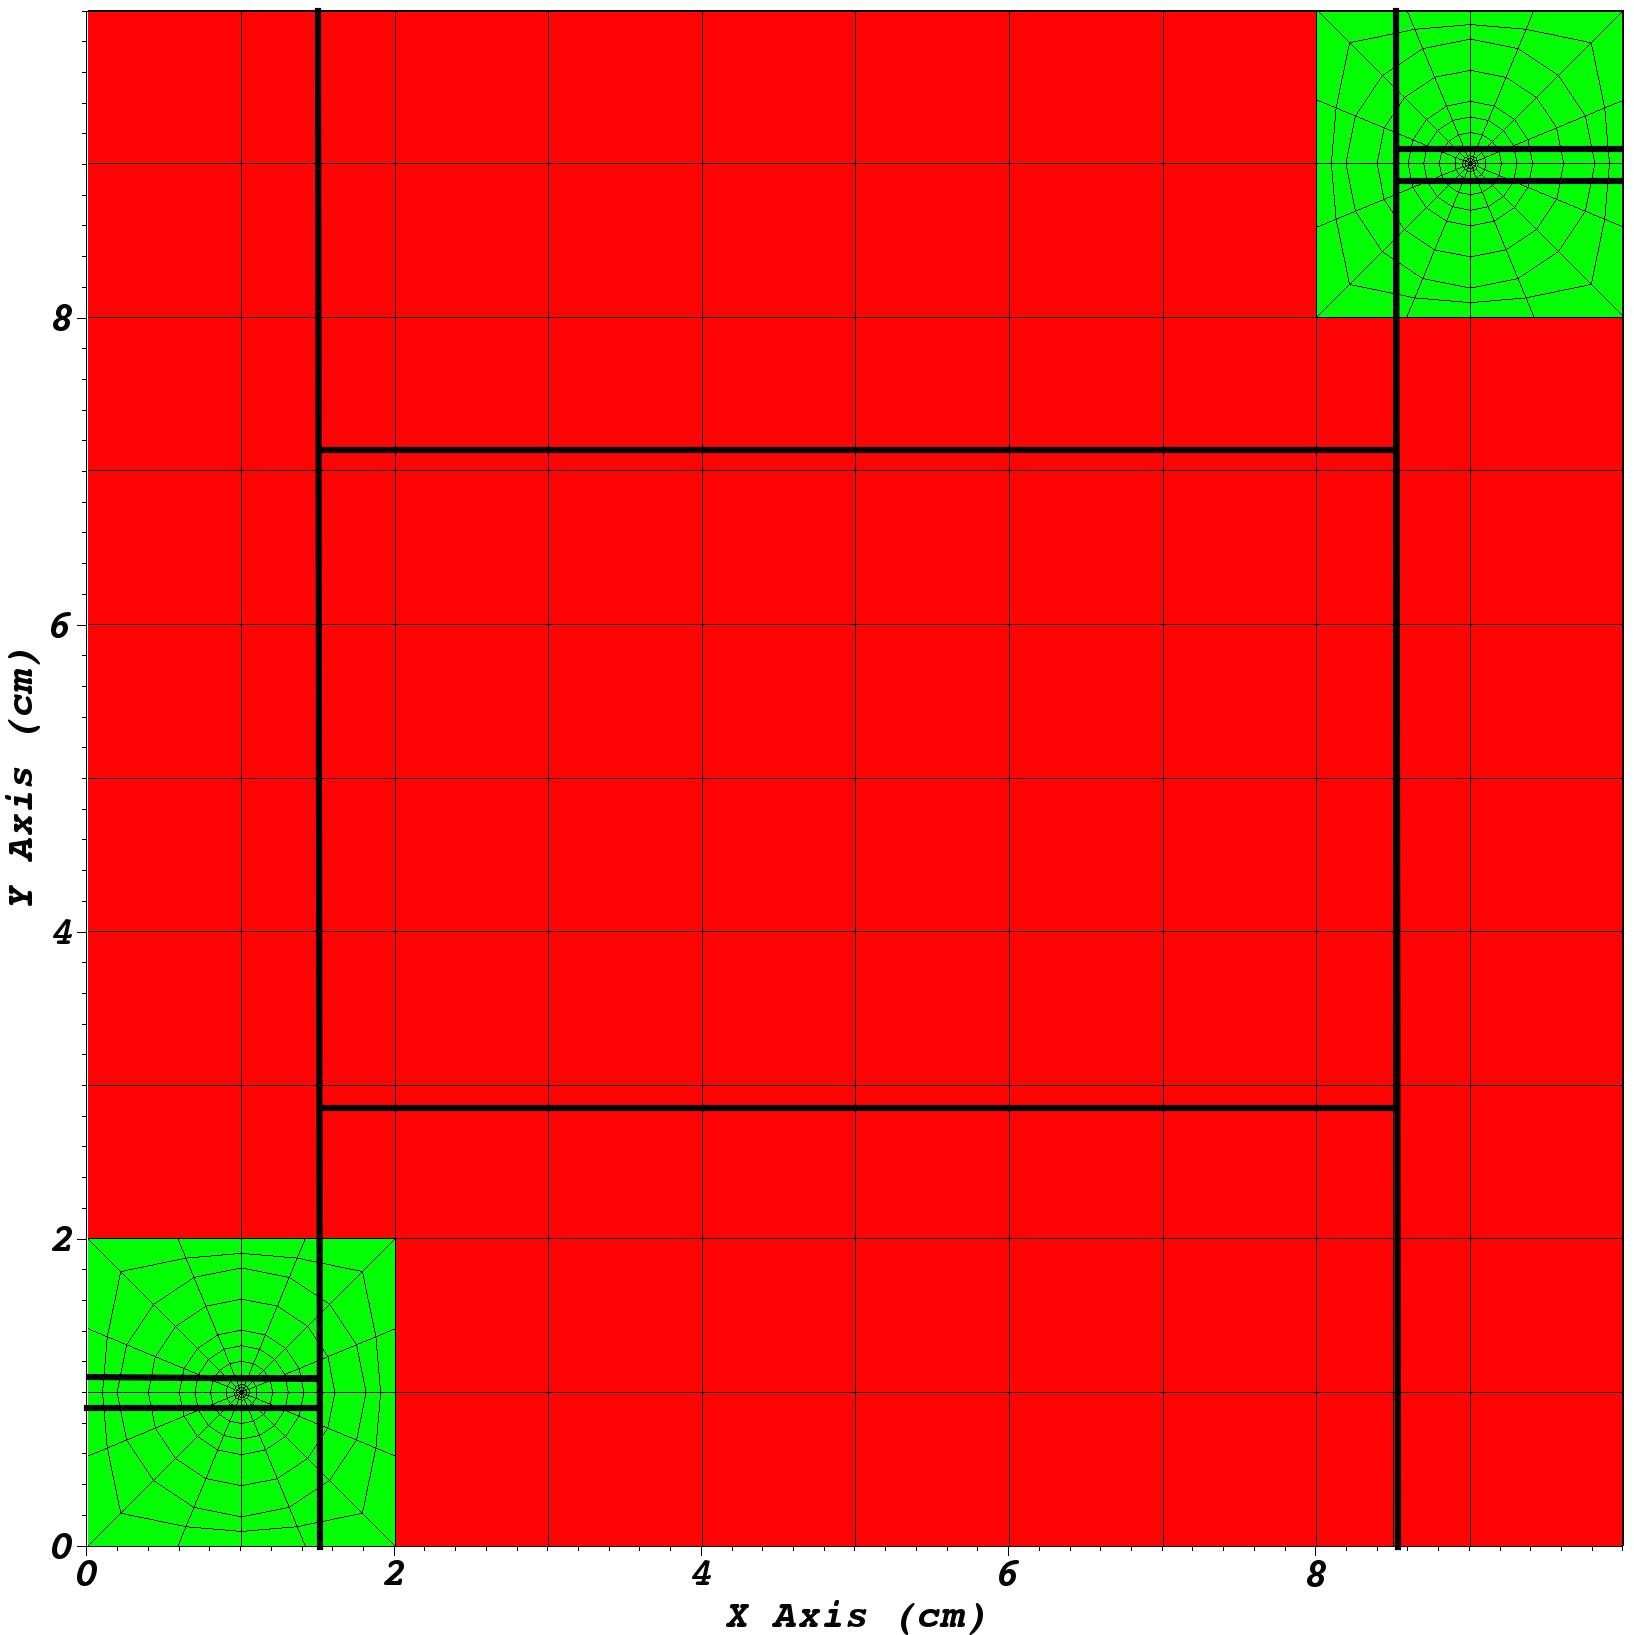
\includegraphics[scale=0.13]{../figures/ubp_3x3_lbd.png}
\caption{5 load-balancing-by-dimension iterations, $f = 1.49$.}
\label{3x3_lbd}
\end{subfigure}
\caption{A demonstration of the original load balancing and load-balancing-by-dimension algorithms on an unstructured mesh partitioned into 3x3 subsets.}
\label{alg_illustration}
\end{figure}

\section{Parametric Study of the Original Load Balancing and the Load-Balancing-by-Dimension Algorithms}
To study the behavior and effectiveness of both the original load balancing and the load-balancing-by-dimension algorithm, a parametric study was run on the mesh shown in Fig.~\ref{partitioning_example}.
This mesh was chosen because it is inherently imbalanced as there are two dense geometric features in opposing corners with a sparse region in between.

The study calculates $f$ for the mesh with no load balancing iterations, 5 original load balancing iterations, and 5 load-balancing-by-dimension iterations.
The mesh is partitioned into 2 to 10 subsets in each dimension for all load balancing formats.
Figure~\ref{metric_study} shows the results of this parametric study.
The results are tabulated in Table \ref{metric_study_table}.

With regular cut lines going through the mesh, $f_\text{reg}$ generally increases as the number of subsets increases.
As the number of cut lines increases, the number of cells added may also increase, driving up the maximum number of cells in each subset. It is important to note that in Eq. \ref{metric_def}, the average number of cells per subset used to calculate $f$ is the average number of cells per subset \textit{before} slicing through the mesh.
With more cut lines, the maximum number of cells per subset will increase while the average number of cells per subset will decrease, leading to an increase in $f$. There can be exceptions to this trend, as seen by ${f_\text{reg}}$ for 8 and 10 subsets in each dimension.
The cut lines with 10 subsets in each dimension lie on natural boundaries when evenly distributed.
A natural boundary is a mesh boundary that coincides with a subset boundary, adding no cells to the mesh.
Because no cells are added in the 10x10 case, $f_{\text{reg}}$ with 10 subsets in each dimension is lower than $f_{\text{reg}}$ with 8 subsets in each dimension.

For the load balanced and load-balanced-by-dimension cases, we see a similar increasing trend for $f$, although it is not quite as consistent for the load-balanced-by-dimension cases.
\begin{figure}[H]
\centering
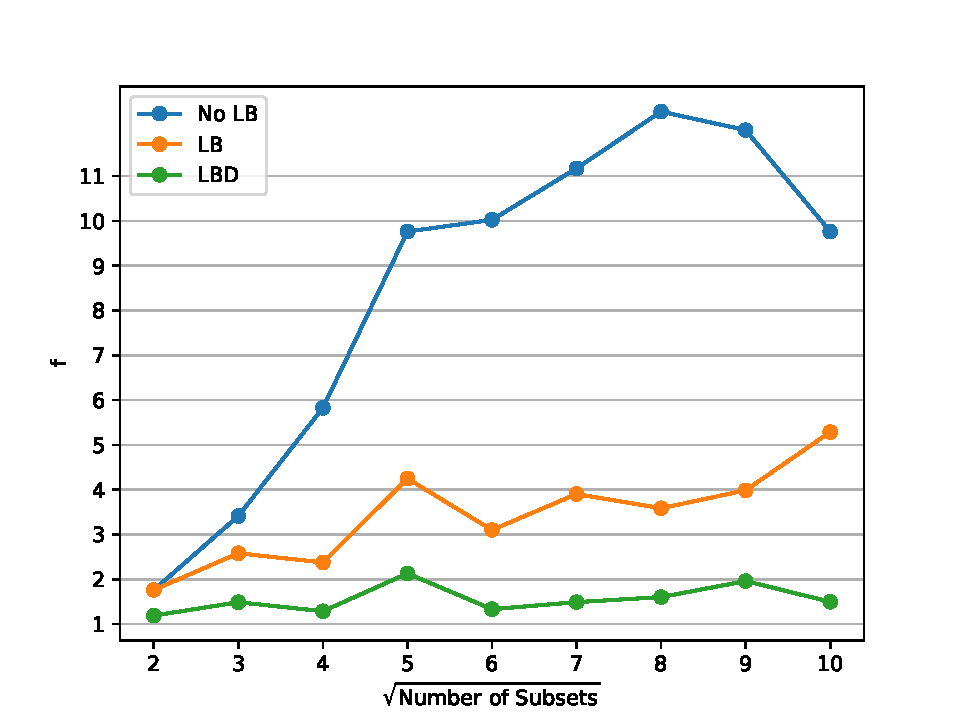
\includegraphics[scale=0.7]{../figures/metric_study.pdf}
\caption{The results of the parametric study with no load balancing, 5 original load balancing iterations, and 5 load-balancing-by-dimension iterations.}
\label{metric_study}
\end{figure}
\begin{table}[H]
\centering
\caption{The tabulated results of the parametric study shown in Fig.~\ref{metric_study} with no load balancing, 5 original load balancing iterations (LB), and 5 load-balancing-by-dimension (LBD) iterations.}
\label{metric_study_table}
\scalebox{0.8}{
\begin{tabular}{c|c|c|c}
\textbf{$\sqrt{\text{Num Subsets}}$} & \bf $f_{\text{reg}}$ & \bf $f_{\text{LB}}$  & \bf $f_{\text{LBD}}$\\ \hline
2&1.76&1.76&1.19\\ \hline
3&3.41&2.58&1.49\\ \hline
4&5.83&2.38&1.29\\ \hline
5&9.76&4.25&2.13\\ \hline
6&10.02&3.1&1.33\\ \hline
7&11.17&3.9&1.49\\ \hline
8&12.44&3.59&1.6\\ \hline
9&12.03&3.99&1.96\\ \hline
10&9.76&5.29&1.5
\end{tabular}}
\end{table}

Table \ref{metric_improvement} shows the percent decrease in $f$ with the original load balancing algorithm and the load-balancing-by-dimension algorithm relative to no load balancing, and the percent decrease in $f$ with the load-balancing-by-dimension algorithm relative to the original load balancing algorithm.
There is consistent improvement for both algorithms for all cases, and the improvement both load balancing algorithms relative to no algorithm generally increases as the number of subsets increases. The improvement of load-balancing-by-dimension over load balancing is notable, with a minimum improvement of 32.43\% and a maximum improvement of 71.66\%.
\begin{table}[H]
\centering
\caption{The percent decrease of $f$ with the original load balancing algorithm (LB) and the load-balancing-by-dimension algorithm (LBD) relative to no load balancing, and the percent decrease of $f$ with the load-balancing-by-dimension algorithm relative to the original load balancing algorithm.}
\label{metric_improvement}
\begin{tabular}{c|c|c|c}
\centering
\textbf{$\sqrt{\text{Num Subsets}}$} & \textbf{LB v. No LB}  & \textbf{LBD v. No LB} & \textbf{LBD v. LB} \\ \hline
2&0.0\%&32.43\%&32.43\%\\ \hline
3&24.38\%&56.38\%&42.33\%\\ \hline
4&59.21\%&77.9\%&45.82\%\\ \hline
5&56.48\%&78.17\%&49.83\%\\ \hline
6&69.05\%&86.7\%&57.01\%\\ \hline
7&65.06\%&86.66\%&61.83\%\\ \hline
8&71.17\%&87.1\%&55.27\%\\ \hline
9&66.84\%&83.69\%&50.81\%\\ \hline
10&45.85\%&84.65\%&71.66\%
\end{tabular}
\end{table}

The same parametric study was run on an experiment that PDT simulates, the Level 2 experiment, shown in Fig.~\ref{level2_nocut_lbchapter}.
\begin{figure}[ht]
\centering
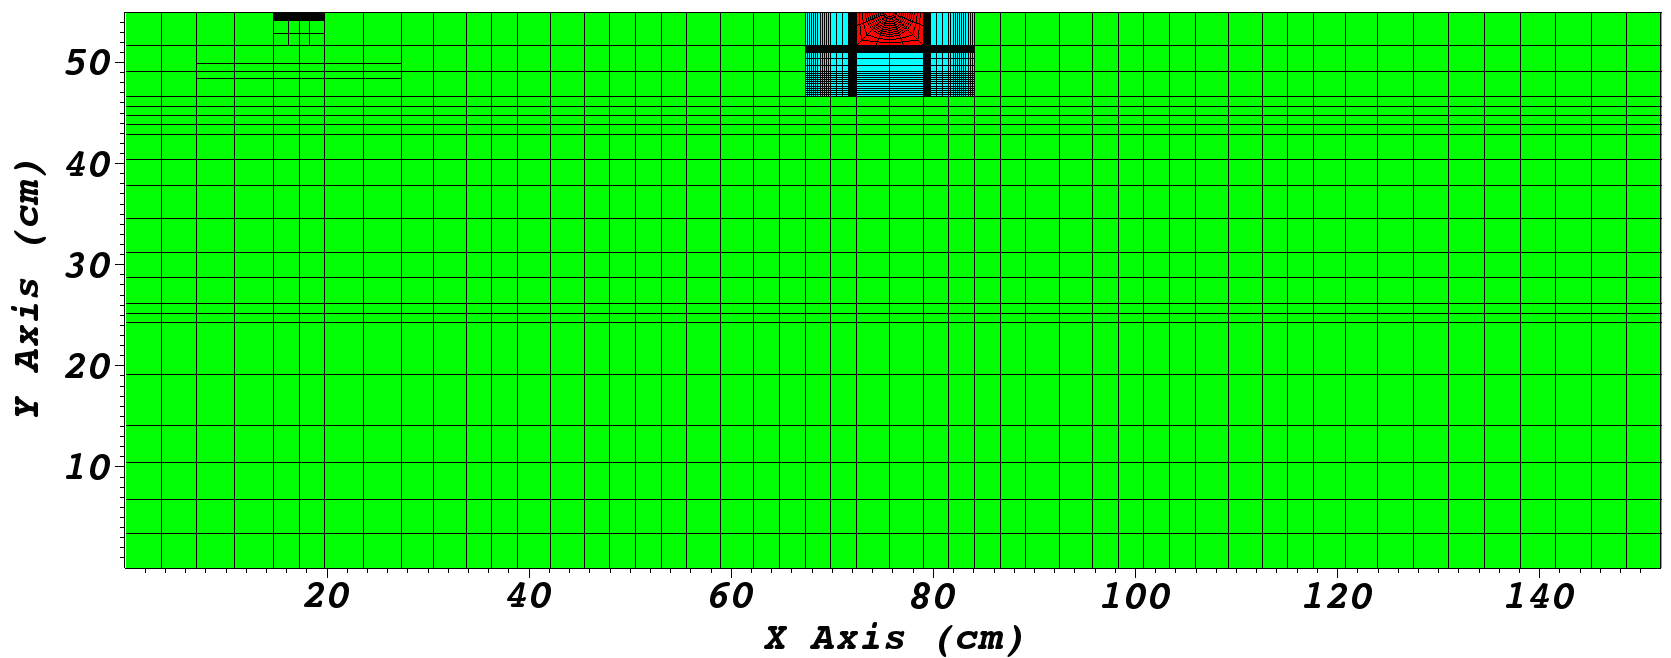
\includegraphics[scale=0.3]{../../figures/level2_nocut.png}
\caption{The mesh for the Level 2 experiment.}
\label{level2_nocut_lbchapter}
\end{figure}
The Level 2 mesh contains a relatively uniform geometry throughout the mesh with one denser feature in the middle of the top boundary.
Figure~\ref{level2_metric_study} shows the results of this parametric study, which are tabulated in Table \ref{level2_metric_study_table}.
%%%%%%%
\begin{figure}[H]
\centering
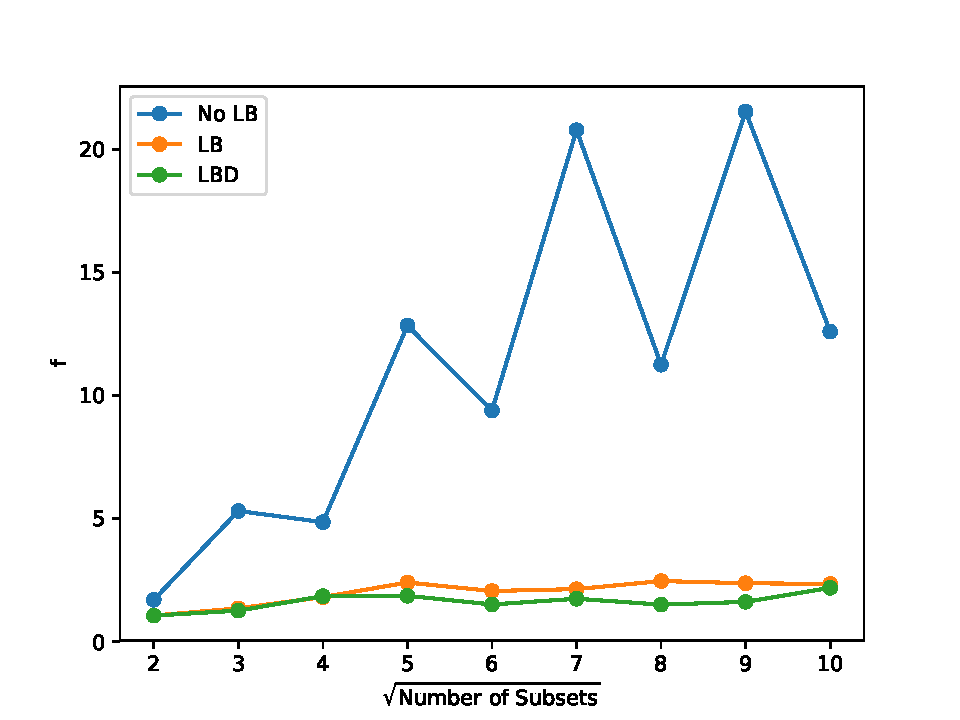
\includegraphics[scale=0.7]{../figures/level2_metric_study.pdf}
\caption{The results of the parametric study with no load balancing, 5 original load balancing iterations, and 5 load-balancing-by-dimension iterations for the Level 2 mesh.}
\label{level2_metric_study}
\end{figure}
\begin{table}[ht]
\centering
\caption{The tabulated results of the parametric study shown in Fig.~\ref{level2_metric_study} with no load balancing, 5 original load balancing iterations (LB), and 5 load-balancing-by-dimension (LBD) iterations for the Level 2 mesh.}
\label{level2_metric_study_table}
\scalebox{0.8}{
\begin{tabular}{c|c|c|c}
\textbf{$\sqrt{\text{Num Subsets}}$} & \bf $f_{\text{reg}}$ & \bf $f_{\text{LB}}$  & \bf $f_{\text{LBD}}$\\ \hline
2&1.7&1.06&1.06\\ \hline
3&5.31&1.35&1.26\\ \hline
4&4.85&1.81&1.85\\ \hline
5&12.83&2.4&1.86\\ \hline
6&9.39&2.06&1.51\\ \hline
7&20.78&2.13&1.74\\ \hline
8&11.25&2.46&1.5\\ \hline
9&21.53&2.37&1.61\\ \hline
10&12.59&2.34&2.18
\end{tabular}}
\end{table}

With regular cut lines going through the Level 2 mesh, $f_\text{reg}$ behaves more erratically than the two pin mesh in Fig.~\ref{partitioning_example}. The natural boundaries are not as uniform, and cells are added in a less consistent fashion. It is noticeable that even numbers of subsets take advantage of the problem's symmetry and consistently have a smaller $f_\text{reg}$ value.

$f_\text{LB}$ and $f_\text{LBD}$ behave much less erratically than $f_\text{reg}$ for the Level 2 mesh.
Table \ref{level2_metric_improvement} shows the percent decrease in $f$ with the original load-balancing algorithm and the load-balancing-by-dimension algorithm relative to no load balancing, and the percent decrease in $f$ with the load-balancing-by-dimension algorithm relative to the original load-balancing algorithm.
Both algorithms can decrease $f$ up to 90\%, but what is notable is the smaller improvement in the load-balancing-by-dimension algorithm relative to the load-balancing-algorithm.
With only one dense feature located in the middle of the mesh, moving the $y$ cut lines on a columnar basis is much less advantageous.
%%%%%%%%%%%%%%
\begin{table}[ht]
\centering
\caption{The percent decrease of $f$ with the original load balancing algorithm (LB) and the load-balancing-by-dimension algorithm (LBD) relative to no load balancing, and the percent decrease of $f$ with the load-balancing-by-dimension algorithm relative to the original load balancing algorithm for the Level 2 mesh.}
\label{level2_metric_improvement}
\begin{tabular}{c|c|c|c}
\textbf{$\sqrt{\text{Num Subsets}}$} & \bf LB v. Regular  & \bf LBD v. Regular & \bf LBD v. LB \\ \hline
2&37.88\%&37.88\%&0.0\%\\ \hline
3&74.56\%&76.29\%&6.8\%\\ \hline
4&62.74\%&61.95\%&-2.11\%\\ \hline
5&81.3\%&85.51\%&22.53\%\\ \hline
6&78.11\%&83.95\%&26.66\%\\ \hline
7&89.74\%&91.62\%&18.33\%\\ \hline
8&78.13\%&86.65\%&38.96\%\\ \hline
9&88.99\%&92.51\%&31.96\%\\ \hline
10&81.41\%&82.66\%&6.71\%
\end{tabular}
\end{table}

\FloatBarrier
The unstructured meshing capability in PDT allows the user to solve a wider variety of problems, without the need to conform a geometry to a logically Cartesian mesh.
The original load balancing and load-balancing-by-dimension algorithms allowed for these unstructured problems to be run more efficiently on large numbers of processors.
However, PDT's performance model does not account for unstructured meshes or imbalanced partitions, but rather assumes a structured grid with an equivalent amount of cells per processor.
In addition, theoretical studies showed that well balanced partitions when using the load-balancing-by-dimension algorithm did not always translate to a better sweep time.
These two reasons motivated the development of a time-to-solution estimator that can estimate the sweep time for a problem given a partitioning scheme ($P_i, A_i$) regardless of mesh type. The time-to-solution estimator is described in Chapter \ref{cha:tts}.

\jcr{can you add for level-2 plots with where the cut lines are placed for regular/LB/LBD?}
